%!TEX root = ../rapport.tex
%!TEX encoding = UTF-8 Unicode

% Chapitres "Introduction"

% modifié par Francis Valois, Université Laval
% 31/01/2011 - version 1.0 - Création du document

\chapter{Avancement de la conception et de la construction du système}
\label{s:avancement}
\section{Alimentation des périphériques 5V}
L'alimentation employée pour les périphériques est une alimentation de type buck qui convert la tension de la batterie (11.1V) vers une tension usuelle de 5V. Cette alimentation utilise un hacheur de tension avec une fréquence autour de 50kHz. Cette fréquence procure une marge de sécurité par rapport à la fréquence d'antenne et évite l'ajout d'un bruit excessif. Cette alimentation a été réalisée avec succès, les plans sont présentés à la figure \ref{fig:alim5V}. Une photo de ladite alimentation est présentée à la figure \ref{fig:alim5Vphoto}.

\begin{figure}[htbp]
\centering
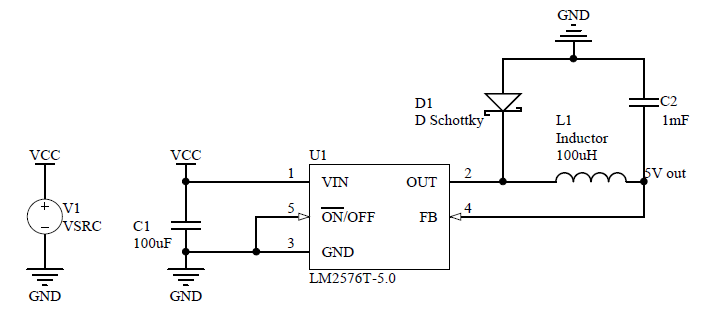
\includegraphics[scale=0.5]{fig/alim_5V.png}
\label{fig:alim5V}
\caption{Figure présentant les plans de l'alimentation 5V pour les périphériques}
\end{figure}

\begin{figure}[htbp]
\centering
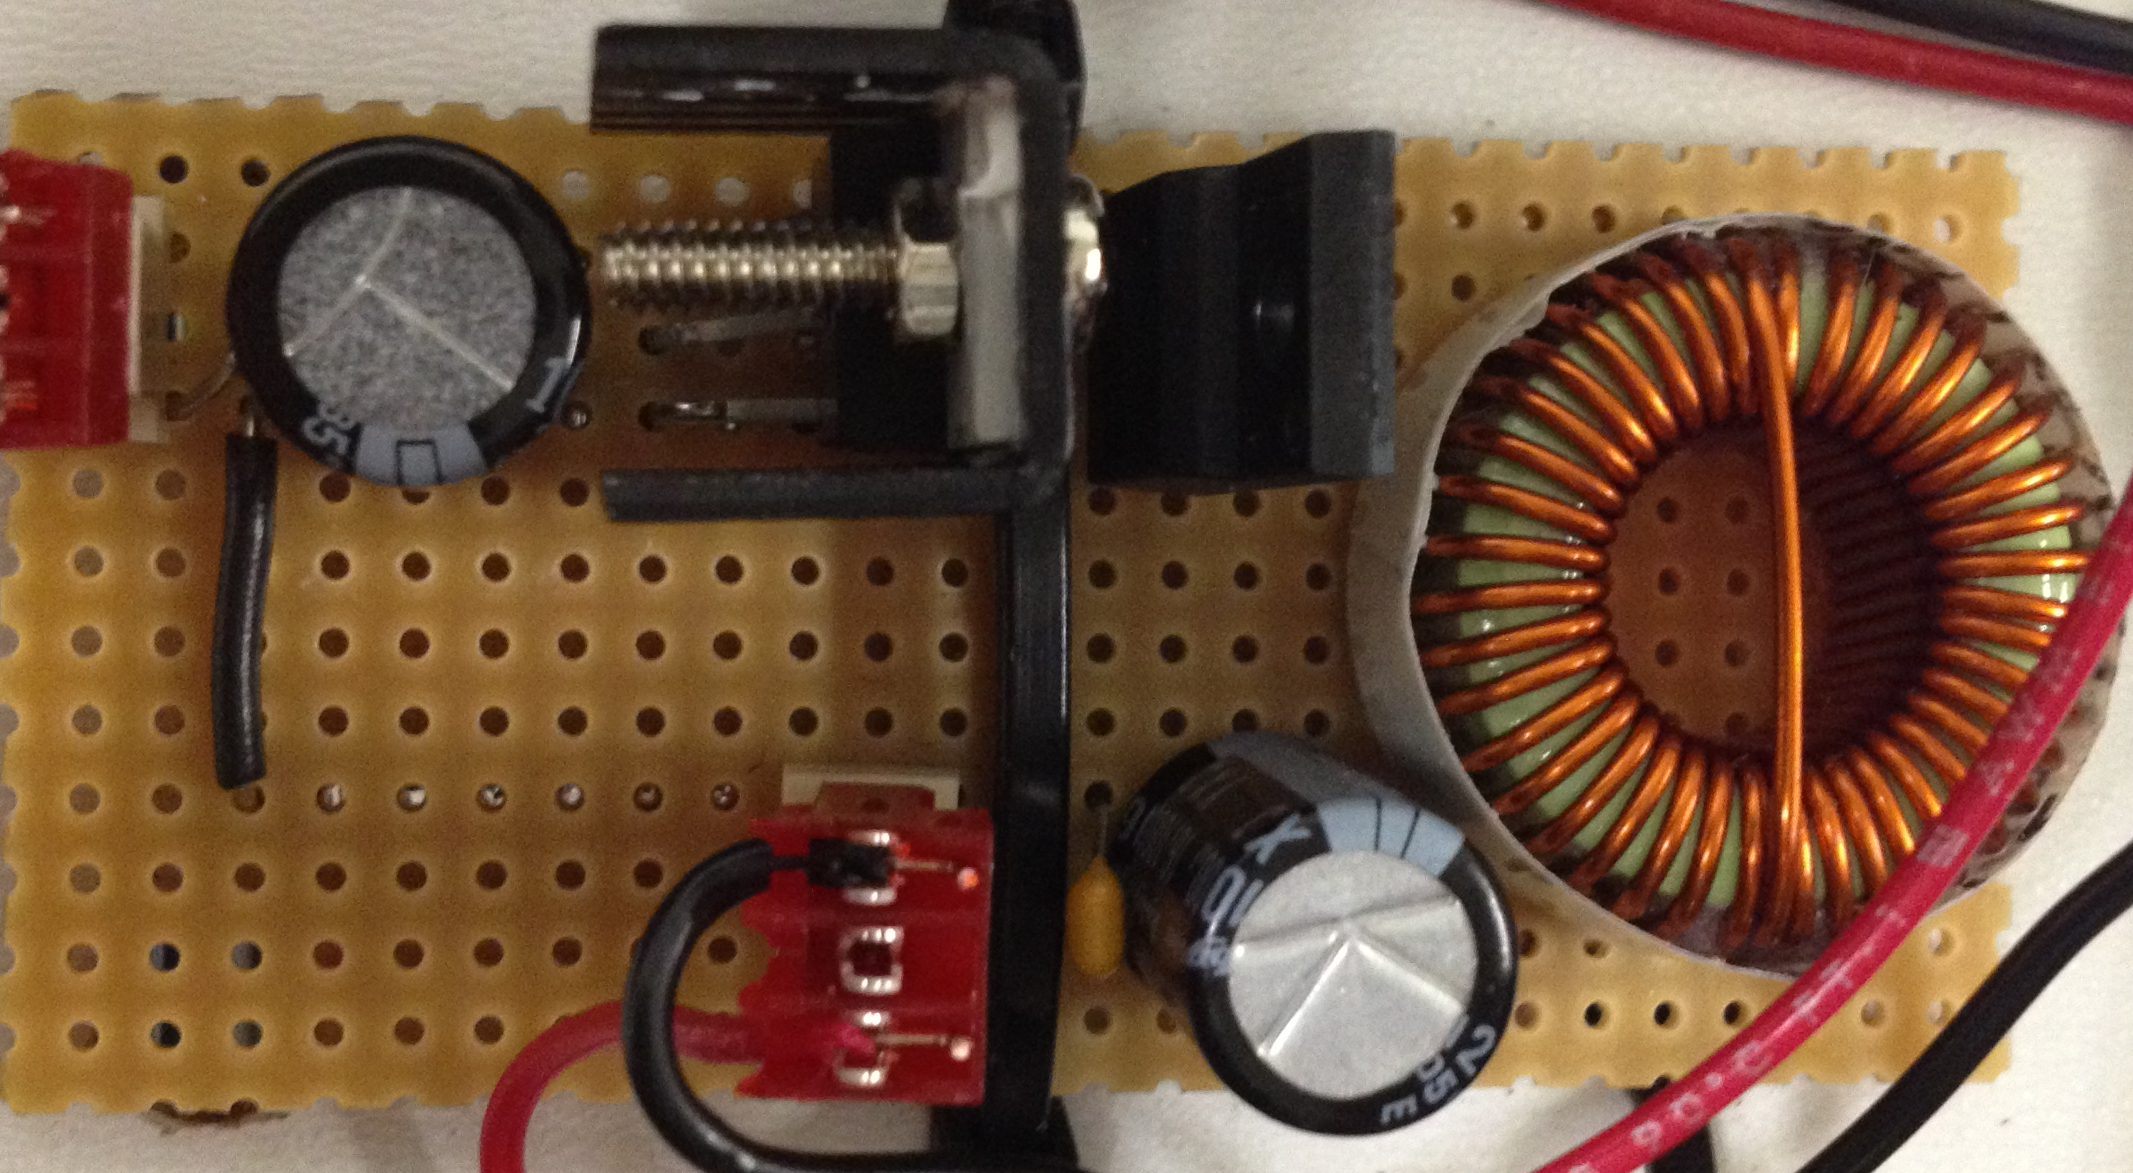
\includegraphics[scale=0.2]{fig/alim_5V_photo.png}
\label{fig:alim5Vphoto}
\caption{Figure présentant une photo de l'alimentation 5V pour les périphériques}
\end{figure}

\section{Alimentation du Mac mini}
L'alimentation du Mac mini a été réalisé au moyen d'un circuit de type Boost réglable, acheté déjà monté. Les plans ne sont pas disponibles, mais une photo du dispositif l'est à la figure \ref{fig:alim24Vphoto}.

\begin{figure}[htbp]
\centering
\includegraphics[scale=0.1]{fig/alim_24V_photo.png}
\label{fig:alim24Vphoto}
\caption{Figure présentant une photo de l'alimentation 24V pour les périphériques}
\end{figure}

